\section{Dati senza Intervalli}

Devi utilizzare questa sezione solo quando hai dei dati \textbf{Senza
    Intervalli}, devi anche fare attenzione che il \textbf{numero di osservazioni $n
        > 30$}!!\\

Calcoli da effettuare:

\begin{enumerate}
    \item Riportare i dati in una tabella in Calc:
          \begin{itemize}
              \item \textit{Colonna 1}: $categorie$
              \item \textit{Colonna 2}: $f_i$
          \end{itemize}
    \item Raggruppare le categorie se $\exists \ categoria < 5$:
          \begin{itemize}
              \item Parti dall'ultimo a salire (dal basso verso l'alto delle
                    categorie)
              \item Raggruppale tutte nell'ultima categoria che le faccia
                    diventare maggiori di 5 sommando le frequenze.
              \item \textit{Esempio}:
                    \begin{figure}[H]
                        \centering
                        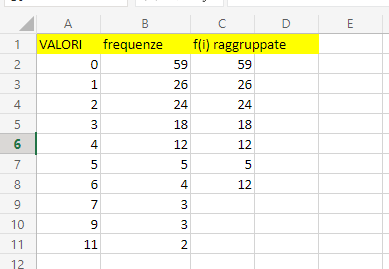
\includegraphics[width=6cm, keepaspectratio]{capitoli/goodnes_of_fit/imgs/vesceragay.png}
                        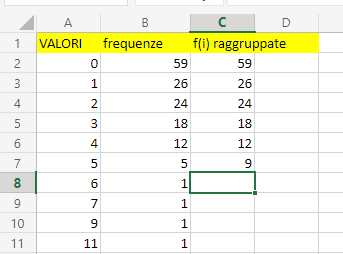
\includegraphics[width=5.5cm, keepaspectratio]{capitoli/goodnes_of_fit/imgs/POSTAMOLTOGAY.png}
                    \end{figure}
          \end{itemize}
    \item Calcolare:
          \begin{enumerate}
              \item n = $\sum(frequenze)$
              \item \st{$f(i) = f_i / n$: non serve}
              \item $p(i)$: dipende dalla distribuzione, vedere AGGIUNGERE
                    REF
              \item $F_i = n * p(i)$: numero di intervalli unitari teorici
                    con $i$ arrivi
              \item $G_i = \frac{(f_i - F_i)^2}{F_i}$
              \item $V = \sum G_i$: sommare tutti i valori di $G$
              \item $df = \text{Numero Categorie} - 1 - \text{Numero
                            Parametri Distribuzione}$
          \end{enumerate}
\end{enumerate}

Una volta terminati i calcoli devi guardare la riga nella tabella del $\chi^2$
(AGGIUNGERE REF) con lo stesso valore di $df$: devi controllare che il valore
$V$ ricada negli intervalli che non superino il $P_{95}$.
